% Chapter 1

\chapter{Background} % Write in your own chapter title
\label{Background}
\lhead{Chapter 1. \emph{Background}} % Write in your own chapter title to set the page header


\section{Provenance of Electronic Data}

A significant factor when buying a piece of artwork is the knowledge of the derivation of that item, as well as, the chronology of the ownership. This has been extensively described with the term provenance and is important for various reasons, chief of which is the fact that it can help us trace the whole history of an object and thus determine the authenticity and establish its historical importance.  Ultimately, one can use this information to determine the value of a work of art.
The same concept has been applied to digital resources or digital information that is generated by computer applications [5]. More specifically, in computer science, we refer to provenance of a piece of data, as the process that led to that specific piece of data [1]. Moreover, any other data or hardware or user interaction that took part in the computational process, belong to the provenance of that piece of data. In general though, the description of such derivation may be represented in any form based on users' personal interest [9].

\subsection{Provenance in Scientific Workflows and Curated Databases}

Substantial work on provenance of data has been undertaken by the database, workflow [6:5, 6:9] and e-science communities.  In particular, the provenance of scientific results can provide proof about the correctness of a result and determine the amount of trust one can place on it [5]. Representative examples are workflows in the scientific domain. A workflow [e.g. myGrid/Taverna [6:18], Kepler [6:6], visTrail [6:13], chimera [6:12] etc], essentially, has been proved to be a successful way to perform complex data processing tasks. Figure 1.1, illustrates an abstract view of a typical workflow. Boxes are used to indicate data processing steps and arrows illustrate the data flow. Each task may take input data from the preceding task, user interactions or external sources (database, external tools).  During a typical workflow run, the means (e.g. input data, user interactions, user parameters etc.) that are involved in the actual derivation of a result, are not recorded whatsoever.  However, the lack of such provenance information makes the outcome of complex analysis difficult to interpret and reproduce. Thus making these systems provenance-aware will address several issues they suffer from. First of all, scientists will be able to evaluate the correctness of the final workflow output and avoid the duplication of efforts. Furthermore, such provenance information might cater with means for quick troubleshooting or even optimize the whole workflow process [1:278].

\begin{figure}[htbp]
	\centering
		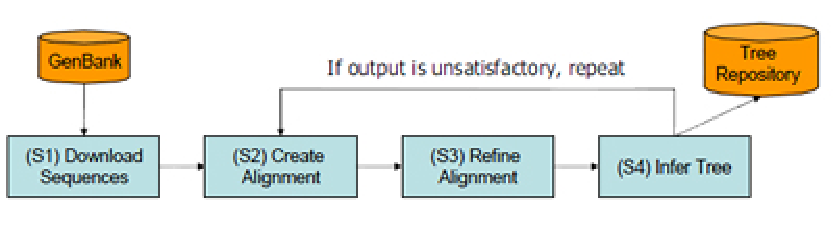
\includegraphics{./Figures/figure1.pdf}
		\rule{35em}{0.5pt}
	\caption[Scientific Workflow]{Scientific Workflow. [6]}
	\label{fig:scientificWorkflow}
\end{figure}


Provenance of data was regarded as an important aspect of the databases storing scientific data. The majority of such databases are usually views of some bigger databases that store raw experimental data. In particular, several scientific stores are populated by the result of queries made to other databases, and are manually updated by several other experts. This sort of databases are commonly known as curated databases [1:53], due to the number of people and/or systems involved in the data insertion and update process. Thus, we can come to recognize that keeping provenance information can help to a great extent to understand the origin of a piece of data, and particularly the process that led to that piece of data. Eventually, we will be able to determine the accuracy, integrity and trustworthiness of data [3].
In the scope of databases, there are two types of provenance that can be observed: "where-provenance", "why-provenance" [3:7]. The former identifies the tuples that were involved in the production of a query result; whereas the latter helps identify the original location a piece of information was copied from.

Consider the following example

\begin{figure}[htbp]
	\centering
		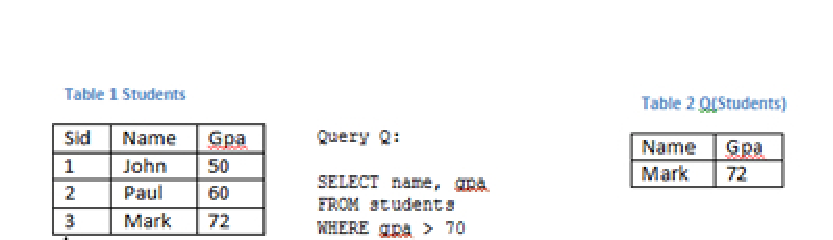
\includegraphics{./Figures/table.pdf}
		\rule{35em}{0.5pt}
	\label{fig:scientificWorkflow}
\end{figure}


Where-provenance can answer to a question such as, where the value gpa ' 72 in the tuple $(mark, 72)$ comes from. The answer would be, that it comes from the field gpa of the tuple with id = 3, in the students table.  Similarly, the why-provenance identifies that the tuple $(3, Mark, 72)$ was the one that contributed to the tuple $(Mark, 72)$ of the query result.
There is a third type of provenance which is called "how-provenance" [1:188]. While why provenance identifies the source tuples that justify a query result, how-provenance goes a step further and tries to describe how those tuples were involved in the creation of that result.

\subsection{Provenance Techniques}

In this section we present a classification of different methods that have been used to support data provenance. Figure 1.2 summarizes the five main aspects according to which we can classify the techniques for data provenance that have been proposed for use in individual domains. [4]

\begin{figure}[htbp]
	\centering
		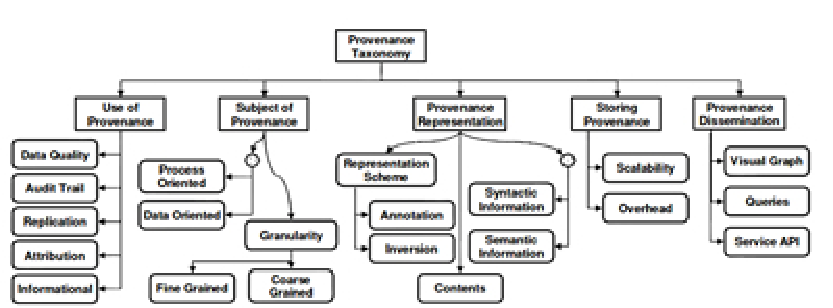
\includegraphics{./Figures/figure2.pdf}
		\rule{35em}{0.5pt}
	\caption[Taxonomy of Provenance]{Taxonomy of Provenance. [4]}
	\label{fig:provTaxonomy}
\end{figure}


\subsection{Applications of Provenance}

As we have already observed, provenance of data can be used for numerous reasons. A good summary the diversity of applications of data provenance is presented by Goble [4:14] and briefly described in the following lines:

\begin{description}
  \item[Data quality]
        Scientific databases and workflows, we examined earlier, belong to this category. Such systems sustain provenance information in order to help users reason about the quality, integrity and reliability of a piece of data.
  \item[Audit trail]
        Provenance can be considered as a logbook tracking all the steps (i.e. process execution details), resources (e.g. hardware, software, input data) and agents (e.g. users, external tools etc.) that were involved in the derivation of a piece of data or a computational result. This information can be useful twofold; locating possible reasons for the existence of an error and for determining resource usage. [4:8]
  \item[Replication recipes]
        Just as is the case in scientific workflows, keeping track of how a computational process was performed, can be useful for validating the results by repeating the same execution.
  \item[Attribution]
        Provenance can be used to tackle the problem of attribution which various systems (e.g. curated databases) usually suffer from [1:53]. More specifically, systems where different users can perform update actions to a dataset, provenance can help attribute the ownership and find the original creator of a piece of data.
  \item[Informational]
        Systems were data are the result of the execution of a sequence of complex tasks (e.g. scientific workflows), provenance is a mean for interpreting data-intensive analysis [6].
\end{description}

\subsection{Subject and Granularity of Provenance Information}

When designing a provenance-aware system, one should specify the subject of provenance - the provenance of what? -  as well as the level of information detail.

Yogesh, et al. [4] introduce two models of provenance: in a data-oriented model, the provenance of data is compiled explicitly in the form of metadata. For example, a directed acyclic graph (DAG)  [1:298] can explicitly present the provenance of a piece of data, by simply describing the process that led to its current state.  Contrary to that, the process oriented model suggests that the deriving processes are entities for which provenance is recorded.  Hence the data provenance is implicitly determined by examining the inputs and outputs of those processes.

The granularity refers to the smallest piece of information that provenance is tracked for. For example, in a relational database we can decide to track provenance to the level of rows or cells. Essentially, the system requirements need to determine the level of granularity.


\subsection{Provenance Representation}
There are two major approaches for computing data provenance [5]: (i) non-annotation (or inversion method) approach and (ii) annotation approach.

\begin{figure}[htbp]
	\centering
		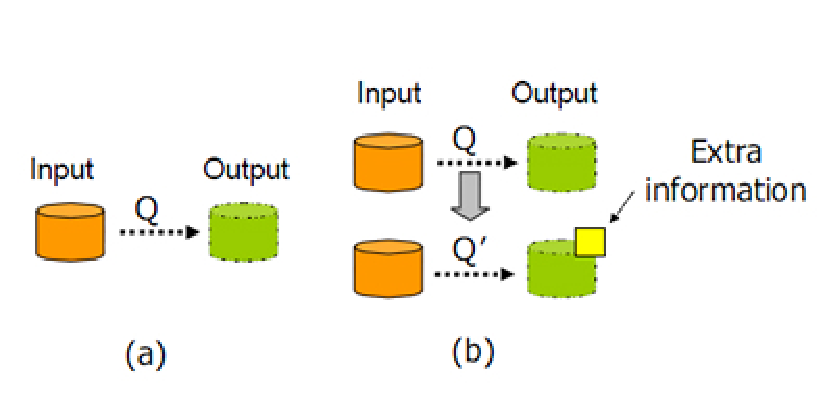
\includegraphics{./Figures/figure3.pdf}
		\rule{35em}{0.5pt}
	\caption[Provenance Represantation]{(a) Non-Annotation (NA) approach, (b) Annotation (A) approach. [5]}
	\label{fig:provRepresentation}
\end{figure}

Consider the example in figure 1.3a.  Q is the transformation function (i.e. query) that acts upon an input database with the aim to generate an output database. This is an example of a non-annotation approach whereby the provenance of the data product (i.e. output database) is computed by analyzing the input and output database, and the definition of Q (e.g. by analyzing the underlying algebraic structure of the query [6:18]). On the other hand, the annotation approach is slightly different. Provenance is determined by collating extra information in the form of annotations and descriptions about other resources. In this approach, provenance is serialized in a machine readable format (e.g. xml, rdf/xml).



\subsection{Provenance Dissemination}

Regardless the representation format of provenance, one should be able to view and act upon this captured information. A system needs to provide access and present provenance in both, a user and machine friendly manner. A common way is to visually represent provenance graphs. However, there is a significant caveat. Big provenance graphs are not intuitive and make it difficult for a user to interpret. Hence, this approach is not scalable. A better solution is to support a query engine which can extract smaller parts of a provenance graph.

\subsection{Provenance open data models}

In the previous section we examined how provenance systems have been integrated within scientific workflows and database management systems. Such systems, though, have full control of the information they process and store and thereby they track provenance within their own scope. Architecture like that, promotes tight coupling between the various systems components (e.g. provenance system, execution environment etc.) [8]

In the era of distributed systems, interoperability is a significant factor that needs to be considered. To that end, systems should adopt mechanisms and techniques that utilize open and technology agnostic models. Several approaches for promoting interoperability rely on an infrastructure that supports several provenance stores [8:55, 8:56] which offer long-term persistent storage of provenance information. Nevertheless, the representation of the provenance information should be described in a coherent way, regardless of the technologies involved.

The intent of this section is to summarize some early attempts for designing a common provenance model, as well as, the current W3C provenance data model (by the time of this writing, the W3C provenance working group1 has published a working draft of the specification)


\subsubsection{Provenance in Service Oriented Architecture (SOA)}

Service oriented architecture (SOA) is an architectural style that has been successfully used in distributed systems. The major advantage of a SOA based system is the loose coupling between the various software components, which minimizes the system development time, as well as, the maintenance cost. Applications following the SOA approach are mainly composed dynamically by utilizing services available in a network [SOA reference]. Thus, the need of a shared and technology-agnostic data model is critical for such systems to be able to manage provenance information.

One of the early attempts to integrate provenance systems into SOA applications was the PASOA approach [mash-ups]. According to the PASOA model, provenance information is described with the notion of proves assertions (p-assertions) [9]. P-assertions are, essentially, assertions made by individual services about their involvement in a process execution. Furthermore, they are the main constituents of a process documentation, which in order, provides with description about what happened at execution time (e.g. which algorithms, data sets or services were involved).

Something that is noteworthy at this point is that the full details of the process that brought a data item to its current state, can considerably huge (theoretically can trace back to the big bang [1]). For example, the full provenance of a result produced by a service that calculates the carbon footprints of individuals might include descriptions of the algorithms that were used, users' input, carbon emission calculation methods, data compiled by external devices (e.g. Gps) and so forth. However, this amount of information might be frustrating for a user who wants to obtain the provenance of a specific piece of data. This fact unveils the need of a query engine where users can provide with customized queries, so that they can get the information they need and avoid the information overload.

During a process execution, there are various tasks carried out. For example, different services might interact with each other by exchanging messages (e.g. SOAP messages) or a single service might apply different transformation functions to input data. As a result, the content of p-assertions can vary. We have three distinct categories of p-assertions based on the content of the provenance information that is being captured.

\begin{description}
  \item[Interaction p-assertions]
         It is an assertion that describes how data flows among the various services in a SOA system. An interaction p-assertion consists of an interaction key that identifies an interaction (i.e. source and destination services), as well as, the content of the message itself (e.g. content of SOAP message)
  \item[ Relationship p-assertions] 
      Assertions about how data slows throughout a single service. They can essentially, describe the function or algorithm that was applied to input data, in order to produce the output message.
       Example p19 from architecture for provenance

  \item[Service-state p-assertions]
        During a single execution, a service has a specific internal state. For example, information such as, CPU time used by a service, available space on the disk, user logged in, local time, might be useful to make various interpretations about the computational result.  P-assertions demonstrating all these information are called service-state p-assertions.
\end{description}

The aforementioned p-assertions describe the steps in the history of a process execution and can be visualized as directed acyclic graphs (see figure 1.4)

\begin{figure}[htbp]
	\centering
		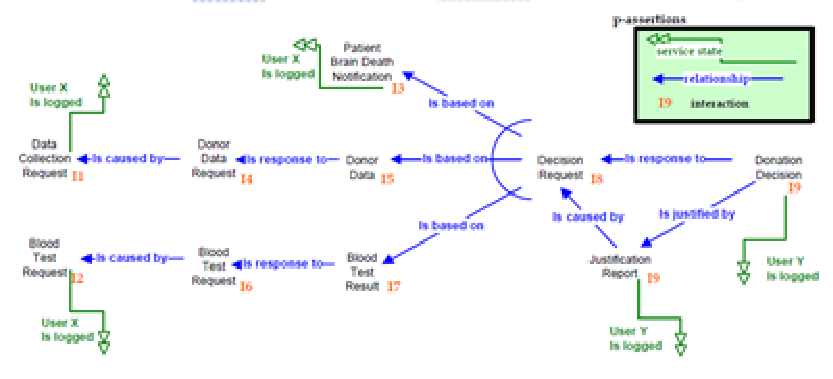
\includegraphics{./Figures/figure4.pdf}
		\rule{35em}{0.5pt}
	\caption[Provenance Directed Graph]{Provenance Directed Graph [9]}
	\label{fig:provGraph}
\end{figure}


\paragraph{Provenance life-cycle}

In this section we briefly describe the different phases that constitute p-assertions life cycle [10]. More specifically, p-assertions pass through four distinct phases, which we outline below.
\begin{enumerate}
  \item
        \textbf{Creating p-assertions:} As we have already mentioned, services are responsible for creating p-assertions while execution precedes each service can only describe its own involvement in the process execution.
  \item
        \textbf{Recording p-assertions:} A provenance store, as described earlier, offers a long-term persistent storage for p-assertions. Hence, after they are created, p-assertions have to be stored in a provenance store, for future use.
  \item
        \textbf{Querying p-assertion:} A provenance store offers a helpful mechanism for obtaining the provenance of a specific piece of data. More specifically, a user can compose queries that will bring the p-assertions according to the users need. In essence, the query will be executed over a process documentation that embraces all the p-assertions.
  \item
        \textbf{Managing p-assertions:} P-assertions may be stored in a provenance store for a long period of time. They therefore may need to be managed over the course of time.
\end{enumerate}

A complete provenance system has to support all these phases of the provenance life-cycle.

\paragraph{A Conceptual Provenance Architecture}

In the previous section we outlined the four main phases of the provenance (or p-assertion) life cycle. For a system to be able to support those phases, a logical architecture that will consist of appropriate system components, has to be designed. Groth et al. [10] suggest generic provenance system architecture (see figure 1.5).

\begin{figure}[htbp]
	\centering
		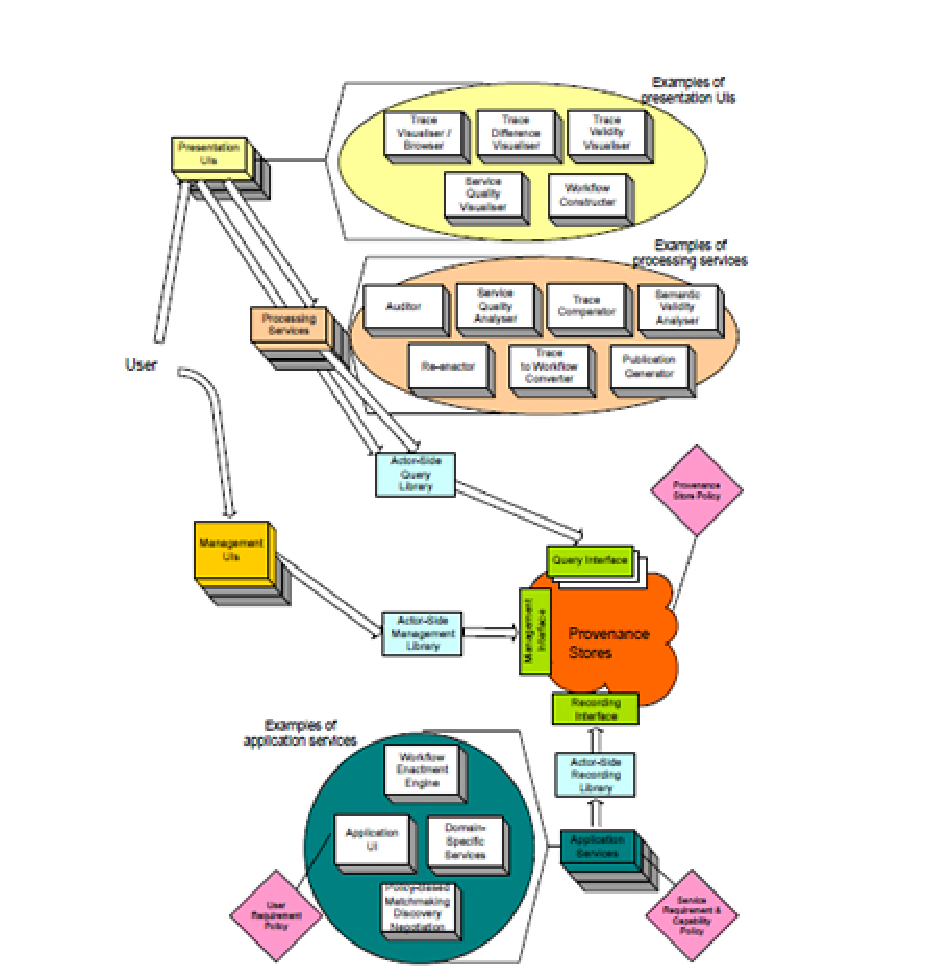
\includegraphics{./Figures/figure5.pdf}
		\rule{35em}{0.5pt}
	\caption[Architecture of Provenance-Aware Application]{Architecture of Provenance-Aware Application. [10]}
	\label{fig:provArch}
\end{figure}

In this architecture, we can observe four different actors that are involved in the provenance life-cycle

\begin{description}
  \item[Application actor] 
        It is the system component that processes the business logic of the application.
  \item[Provenance store] 
        This is the central point in the architecture. As we have already described, it is the responsibility of the provenance store to persist and provide access to the recorder provenance information.
  \item[Querying actor] 
        This is the part of the system that communicates with the provenance store by issuing provenance queries.
  \item[Recording actor] 
        While the querying actor send queries to the provenance store, the recording actor populates it by submitting p-assertions. 
  \item[Asserting actor] 
        This is the actor that creates appropriate p-assertions while the execution proceeds.
  \item[Managing actor] 
        An actor that performs all the managing tasks in the provenance store.
\end{description}

It is obvious that the provenance store is the key actor in the provenance lifecycle. It interacts with several other system components and therefore should provide appropriate interfaces to facilitate those interactions.

\begin{itemize}
  \item 
        A \emph{recording interface} which give access to recording actors so that they can submit p-assertions.
  \item 
        A \emph{query interface} which is the entry point for query actors so that they can issue provenance queries and get back the query results.
  \item 
        A \emph{management interface} which allows managing actors to perform managing tasks in the store.
\end{itemize}

    
\subsubsection{Open Provenance Model}
The provenance data model we presented earlier, describes a shared models for capturing, recording, exchanging and managing provenance information. However, it is primarily bound to SOA applications, that is, to message exchanging systems. The models that we discuss in this section is the first purely technology agnostic provenance data model.

The Open Provenance Model (OPM) [1:299] addresses different provenance interoperability issues by introducing the notion of the provenance interoperability layer [1].

Figure 1.6 illustrates a big system which consists of several individual applications. Each of these applications is designed to be provenance aware and makes use of its own provenance store. In a system like that, where information flows across different applications, the history of the derivation of a piece of data (i.e. provenance) might reside across several provenance stores. As a result, one would need to query several provenance stores, to form the whole process execution chain. It is the job of the inter-operability layer to conceal the technology diversity of individual applications and expose provenance data in a uniform manner.

\begin{figure}[htbp]
	\centering
		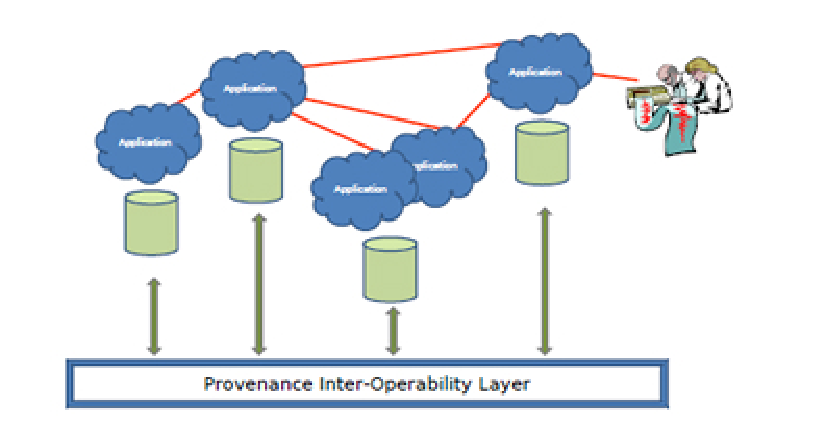
\includegraphics{./Figures/figure6.pdf}
		\rule{35em}{0.5pt}
	\caption[Cross-System Provenance]{Cross-System Provenance. [1]}
	\label{fig:provAccrossSystems}
\end{figure}

The open provenance model utilizes a graph structure to represent a set of causal dependencies [13] among its nodes. A set of such dependencies can explain how a digital piece of data, physical resource (e.g. bicycle) or a conceptual entity (e.g. immaterial entity, idea etc.) came to be in a particular stat at a specified time.

OPM suggests three types of nodes, which we now present:

\begin{description}
  \item[Artifact] 
         A digital, physical or conceptual entity can have different sets of characteristics, at different moments. We call this specific state of an entity, an artifact. An artifact can be viewed as a snapshot of an entity at a given moment. For example, a pdf file at a specific time. States are immutable in that they cannot be modified. Alterations to any characteristic of an entity at a given time result in the generation of a new artifact.
  \item[Process] 
        A process refers to an action or a sequence of actions that result in the generation of new artifacts. For example the process of embedding images into a pdf file produces a new pdf file, enriched with multimedia characteristics (i.e. images).
  \item[Agent] 
        Agent is an entity which triggers a process. in other words, it is the responsibility of an agent to initiate or terminate a process. Following the example with the pdf file, an agent might be a software component that initiated the process of adding images into the new file.
\end{description}

Nodes in an OPM graphs are connected with each other via causal dependencies. Such dependencies are illustrated with directed edges from the source bode (or effect) to the destination node (or cause).

The OPM model introduces an initial set of causal dependencies which are illustrated in figure 1.7. This is a graphical representation of the causal relationships between artifacts, processes and agents. Artifacts are represented by ellipses; processes are represented by rectangles; and agents by octagons. [OPM v1.01]

\begin{figure}[htbp]
	\centering
		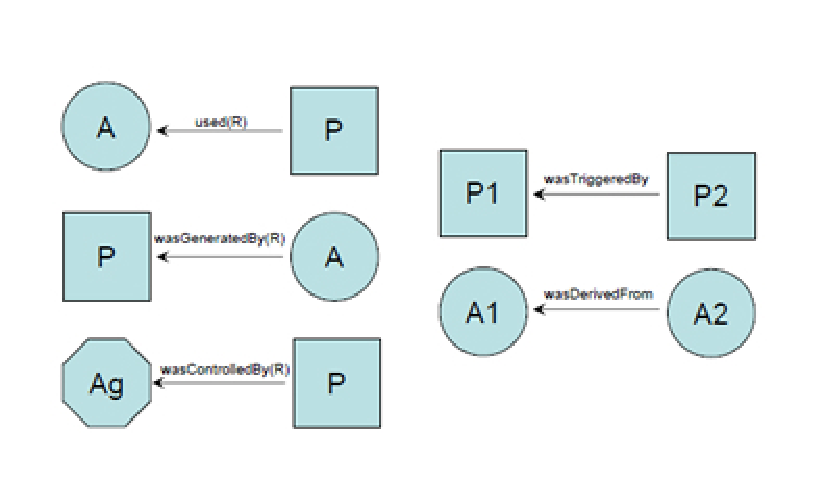
\includegraphics{./Figures/figure7.pdf}
		\rule{35em}{0.5pt}
	\caption[Provenance Causal Dependencies]{Provenance Causal Dependencies [13]. Note that past tense aligns with the notion of process history documentation.}
	\label{fig:provCausalDependencies}
\end{figure}

We observe a set of five types of causal dependencies based on participants.

\begin{description}
  \item[Used] 
        A relationship between a process and an artifact denoting that the process used the artifact to produce a result (e.g. a new artifact). The formal definition suggests that the availability of the artifact is critical for the process to complete the execution.
  \item[wasGenerateBy] 
        It is a relationship between an artifact and a process, indicating that the artifact was generated by the process. In other words, the existence if the artifact is due to the execution of that process.
  \item[wasTriggeredBy] 
        Figure 1.7 shows an edge wasTriggeredBy from a process p2 to a process p1. The semantics of this relationship defines that there was some unknown artifact that was generated by some process p1 and was used by a process p2.
  \item[wasDerivedFrom] 
        An edge wasDerivedFrom from an artifact node A2 to another artifact node A1 denoted that there was a process that used tan artifact A1 to generate an artifact A2. It is a useful relationship, when the actual process of a transformation is unknown.
  \item[wasControlledBy] 
        It is a causal dependency between a process and an agent. It simply indicates that the execution (i.e. the start and end) of a process is carried out under the control of an agent.
\end{description}

Note the letter R in the "used", was controlled by" and "was generated by" edges. This is a bit of extra information that is used in the aforementioned relationships to characterize the role of each entity (i.e. artifacts, agents) that is connected to the same process. More specifically, in a "used" relationship, the same process may use several artifacts. However, the nature of each usage might be different. For instance, an online process for searching for news based on a keyword and a specified source uses the keyword with the role "keyword to search" and the source web site with the role "web site to search". Similarly, a process can generate several artifacts with different role each. Following the previous example, the process can produce a news article and a set of additional sources. The former will have the role "article associated with the keyword" whereas the latter will have the role "additional sources to look at". Finally, a process can be controlled by multiple agents, each with a distinct role. In the example of the online news fetcher, the process for searching news can be initiated either by a user via a user interface, or by an external application via an application programming interface (API). The Roles in this case might be "internal actor" and "external actor" respectively.

One of the concepts associated with provenance that we have been constantly highlighting, is the ability to specify the scope of the provenance that is being captured.  A provenance of a piece of data can be expressed in various levels of detail. Furthermore, it can be viewed from different angles and standpoints. To that end, OPM introduces the notion of accounts [13]. An account is regarded as a graph coloring, indicating different provenance sub-graphs which provide details at different level of abstraction.

P6 figure 10 with accounts

The concept of accounts is fairly useful and caters users with multiple descriptions of the provenance of the same piece of data.
A final note about OPM concerns the extensibility capabilities of the model. Stronger interpretations of the causal dependencies we described in this section can be used to serve application-specific requirements. A common way to achieve that would be to design an ontology with subclasses of those causal dependencies.


\subsubsection{The W3C Provenance Working Group}
The open provenance model was a good initiative to tackle with inter-operability issues pertaining to the provenance dissemination across multiple platforms. However, as is the case of many widely used technologies, there should be a consensus among different bodies (e.g. industry, academia etc.) about the final specification. For this reason, the provenance working group was formed in the World Wide Consortium (W3C). The group followed the work that was started by the Provenance Incubator Group\footnote{$http://www.w3.org/2005/Incubator/prov/wiki/W3C_Provenance_Incubator_Group_Wiki$}. The ultimate goal of the group is to reach an agreement upon the specification of provenance on the World Wide Web.

At the time of this writing, the provenance working group has published a set of specifications which are still on the "working draft" step of the W3C specification approval process. In particular, the specifications that have already been released are:

\begin{description}
  \item[PROV Data Model] 
        A data model for describing all the parties that are involved in the generation of a data item [15].
  \item[PROV Ontology] 
        A OWL 2 web ontology for expressing the PROV data model. In essence, it is the "vocabulary" that is used by the PROV data model to represent provenance information [?].
  \item[PROV Notation] 
        Specification which aims to design the means for a human friendly representation of the information expressed by the Prov data model[?].
  \item[PROV Constraints] 
         A document that defines a set of constraints that assures the validity of PROV instances (statements). Further, it specifies inference rules for reasoning over PROV instances. This can result in the creation of additional statements implied from the explicitly stated provenance information[?].
  \item[PROV Access and Query ] 
        A document that describes the means to leverage the existing web infrastructure, in order to query and obtain provenance information[?].
\end{description}

In this section, we will present the PROV data model (PROV-DM). For additional information about the rest specifications, we refer the reader to the official web site  of the W3C provenance working group\footnote{$http://www.w3.org/2011/prov/wiki/Main_Page$}


\paragraph{PROV Data Model}
Provenance can be viewed from different standpoints, and therefore various kinds of information can be stored in provenance records [14].

The provenance data model identifies three distinct perspectives of provenance:

\begin{itemize}
  \item 
        \textbf{Agent-centered provenance:} emphasis is given on the entities that took part in the generation or manipulation of the data item in question. For example, considering the provenance of a video file in a blog post, we might want to know the person who recorded that video, the person who edited it, and the user who posted it on the blog.
  \item 
        \textbf{Object-oriented provenance:} a different perspective suggests that we might want to identify the origin of different parts of a document. For example, in the same blog post, we may want to know that the video was taken from YouTube and the images from Flickr.
  \item \textbf{Process-oriented provenance:} finally, we may want to highlight the actions that were carried out to generate a data item. For example, a visual graph illustrating the connections I have in a social network site may have been generated by invoking a service to pull data from the social network, which then are processed by a JavaScript library for visualization.
\end{itemize}

Regardless the various viewpoints that provenance can be examined, a good data model should provide all the means needed to capture adequate information. To that end, the PROV-DM introduces some key concepts, which we outline in the following lines.

\begin{figure}[htbp]
	\centering
		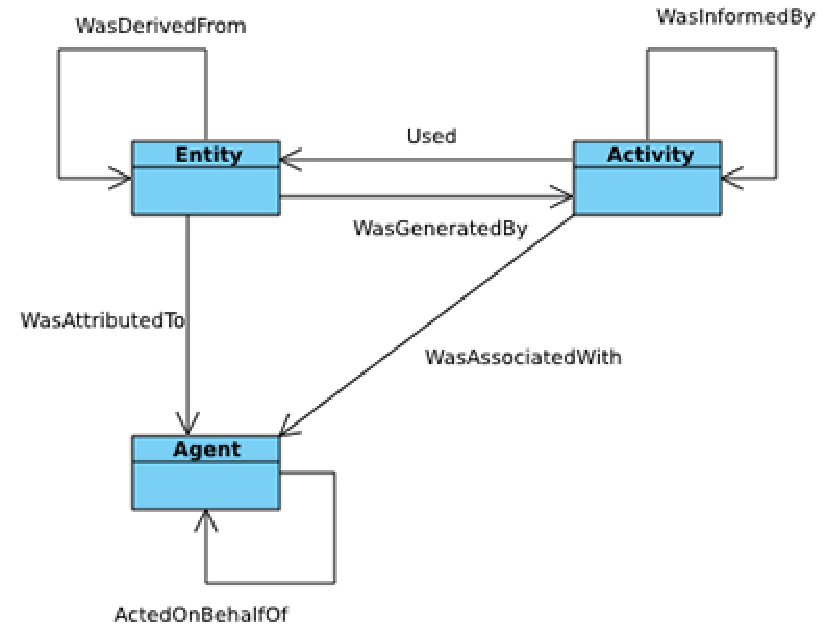
\includegraphics{./Figures/figure8.pdf}
		\rule{35em}{0.5pt}
	\caption[PROV-DM]{PROV-DM [14]. Note that past tense aligns with the notion of process history documentation.}
	\label{fig:provDM}
\end{figure}

An entity is the equivalent to an artifact in the open provenance model. It may refer to a physical, digital or immaterial thing, such as a blog post, a car or a decision. The second, constituent is the activity. This is equivalent to a process in OPM model and represents the derivation of an entity. In particular, it refers to process of generating a new entity or the transformation of one entity to another. For example, the process of calculating the carbon emissions of an individual based on some input data is an activity. Finally, an agent in PROV-DM is assigned a degree of responsibility for an activity that is being carried out. The concept of an agent is similar to that of an actor in the OPM model, in that represents a "thing" that is responsible for controlling the execution of an activity. An agent can be a human being, an organization, software or any other entity that may initiate an activity. For example, a JavaScript visualization library can be an agent that is responsible for imitating a graph visualization activity.

At this point we have to note that provenance can be expressed only for entities. However, we can make provenance assertions about an agent, should the agent be declared both as an agent and an entity.
These are the main concepts of the PROV-DM data model. In addition to that, the data model encompasses several other relationships (for additional information, refer to the official document [15]).


\paragraph{Entity Generation and Usage}

An activity in PROV-DM can be related to an entity in two different ways.  First of all, the effect of the actions that comprise an activity is usually the generation of new entities. Hence, entities exist due to activities existence. For example, assembling car parts brings a car into existence. Additionally, activities can use entities, often during the process of generating other entities. For example, a visualization activity can use some datasets stored in a database, in order to create a chart. These two relationships are represented in the PROV-DM with the terms \emph{wasGeneratedBy} and used respectively

\paragraph{Agents' Responsibility}

Agents can be associated with entities, activities or other agents. Relationships between entities and activities come in the form of responsibility that an agent has over them. We have already highlighted that agents are responsible for the execution of an activity. A responsibility might refer to an agent initiating or terminating an activity. For example, in PROV-DM we say that an activity was associated with an agent. Similarly, an activity can be responsible for an entity. This form of responsibility can be interpreted as the attribution of an entity to an agent. In other words, the was AttributedTo relation, from an entity to an agent, denotes that an agent was responsible for an activity that was the cause for this entity to be created. This is useful relation when the activity is unknown or of a little significance. Finally, PROV-DM provides mechanisms to express relations between two agents. In particular we say that an agent can act on other agent's behalf.  For example, an employee can be designated by the company to perform some actions on their behalf.

\paragraph{Entity Derivation}

The last core relationship defined by the PROV-DM is a relation between two entities. The existence of an entity might often be due to some other entity that was used by the activity that generated it. In that case, it is said that one entity was derived from another entity. A special kind of such relation is the "was revision of". For example, the PROV-DM specification may go through multiple revisions over the course of time. Such relation can be useful to examine the changes that had been brought across the different revisions of a document.

\paragraph{Roles}

Recall the notion of roles in the OPM model. The PROV-DM has adopted the same notion to characterize relationships between entities and activities. In particular, a role specifies how an entity was used or generated by an activity. Similarly, roles can specify the nature of agents' involvement in an activity. It is obvious that roles are application specific, and therefore are not specified by PROV-DM.

\paragraph{Plans and Accounts}

Activities may consist of numerous steps and procedures. For instance, an online tutorial for publishing links data on the web illustrates several steps that should be taken. In PROV-DM there is a specific term to represent this set of actions. In PROV-DM language, this term is called plan. Plans are entities, therefore we can describe provenance for them.
Finally, one would wonder how we can trust the provenance information about a resource. In fact, this is a plausible question, since anyone can make provenance assertions about any entity. The PROV-DM supports a means to address this issue, namely it includes the notion of accounts. In essence, an account is an entity that contains some provenance information, and because it is an entity, we can express a provenance for it. That is to say, provenance of provenance can be expressed.

Example [15]
\begin{verbatim}
Entity(ex:w3c-publication.pn, [prov:type="prov:Account" % % xsd:QName])
wasAttributedTo(ex:w3c-publication.pn, w3:consortium.)
\end{verbatim}

In the above example, which was written in PROV-Notation, we have explicitly declared the "ex:w3c:publication.pn" provenance description. We then state that "w3:consortium" agent was responsible for its generation.

In this section we presented only the core principle of the PROV-DM specification. However, the whole specification is very rich and consists of many more concepts and definitions. For this reason, we would recommend the reader to visit the provenance working group web site to read the whole set of PROV specifications.

\subsection{Security}

A provenance -aware system is, essentially, capable of recording and storing provenance information about different assets that reside in system. As we have already discussed, this sort of functionality is accomplished with the aid of a data model, which defined the way that provenance information is represented internally. Further, the presence of a provenance store guarantees the long-term storage of provenance information, as well as, provides a means for querying the store [19:5]. The result of a provenance query is a causal graph or provenance graph, which illustrated the provenance information in a way that can be viewed an analyzed.

Throughout the process described above, there is nothing that guarantees the quality and integrity of provenance information. To address this problem a framework that will consider all the security-related aspects of the provenance information, have to be devised. Such framework can leverage existing technologies (e.g. cryptography), that have been successfully applied on the web.
We will start our discussion by introducing some fundamental concepts and technologies pertaining to the security in computer systems.

\subsubsection{Fundamental concepts}

A discussion about security issues concerning the communication between different entities, which exchange some sort of information, should start by defining some initial security requirements. More specifically, there are five requirements that a secure system must provide.

\begin{description}
  \item[Confidentiality] 
        A system has to guarantee that all the information that is being exchanged between different entities is protected against eavesdroppers; for example, the information that we exchange when purchasing a product on eBay, should not be wire tapped by anyone.
  \item[Integrity] 
        A message sent from one to entity to other should not be altered, whatsoever; foe instance an order sent to eBay has to remain intact while traveling through the wire.
  \item[Authentication] 
        A mechanism that blocks unauthorized users from accessing the systems data and functionality. Access should be granted only to those users who can provide adequate information, in order to prove their identity; for instance In order to be able to perform a purchase action on eBay, one should provide his credentials.
  \item[Non-repudiation] 
        An important requirement in the communication between two entities is to be able to prove that a message was indeed sent by its sender; for example, once a user submits a purchase order, she cannot claim that has not done so.
  \item[Authorization] 
        This requirement is also known as access control. It, essentially, is a mechanism that determines the sort of access that a user can have on systems resources; for example, as an ordinary user, I cannot modify the systems database by deleting items that I am not authorized to delete.
\end{description}

\subsubsection{Cryptography}

Authorization and authentication are two requirements that can be achieved fairly easier that the rest. To support authorization, a system can simply apply one of the proposed models for access control (e.g. MAC [?], DAG [?], RBAC [?], ABAC [?] etc.). Similarly, authentication can be achieved by leveraging the current web infrastructure and the HTTP protocol capabilities (e.g. content negotiation). To meet the rest requirements, a system can use cryptography technics. More specifically, confidentiality can be ensured with encryption [?] whereas non-repudiation with digital signatures [?]. Finally, integrity can be guaranteed with either of those two technics. We review those technologies in the following sub-sections.

\paragraph{Symmetric Encryption}

This type of encryption requires that the entities that participate in a message exchange communication use the same key for the encryption and decryption phase. For example, figure 1.9 illustrates a message exchange scenario.

\begin{figure}[htbp]
	\centering
		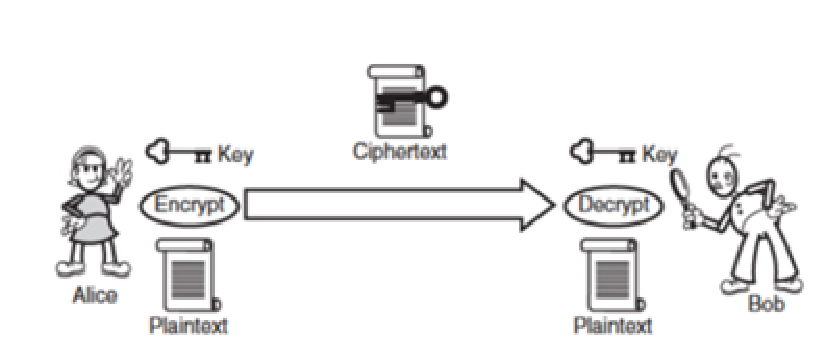
\includegraphics{./Figures/figure12.pdf}
		\rule{35em}{0.5pt}
	\caption[Symmetric Encryption]{Symmetric encryption. [?]}
	\label{fig:symmetricEncryption}
\end{figure}

In this scenario Alice wants to send a message to Bob. As shown in the figure, she encrypts the original data (plaintext) with a private key, and sends it to Bob who decrypts the encrypted message (cipher text) using the same private key. Some of the algorithms that can used to encrypt data are: 3DES, DES, AES, RC4

\paragraph{Asymmetric Encryption}

Asymmetric encryption is more flexible, in that two different keys are used: a private and a public key; for example, figure 1.10 demonstrate the same scenario but now an asymmetric encryption is used. Alice uses Bob's public key to encrypt the plaintext and sends it to Bob, who decrypts the cipher text using his private key.

\begin{figure}[htbp]
	\centering
		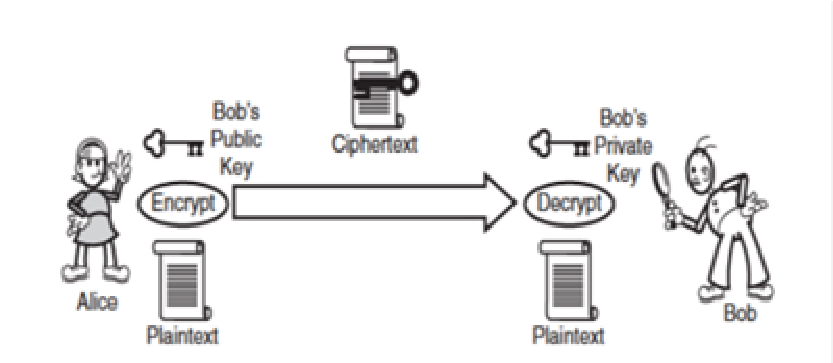
\includegraphics{./Figures/figure13.pdf}
		\rule{35em}{0.5pt}
	\caption[Asymmetric Encryption]{Asymmetric encryption. [?]}
	\label{fig:asymmetricEncryption}
\end{figure}

\paragraph{Digital Signature}

Integrity and non-repudiation can be guaranteed with the use of digital signatures. To better describe this technology look at figure 1.11. Alice has a pair of private and public keys.

\begin{figure}[htbp]
	\centering
		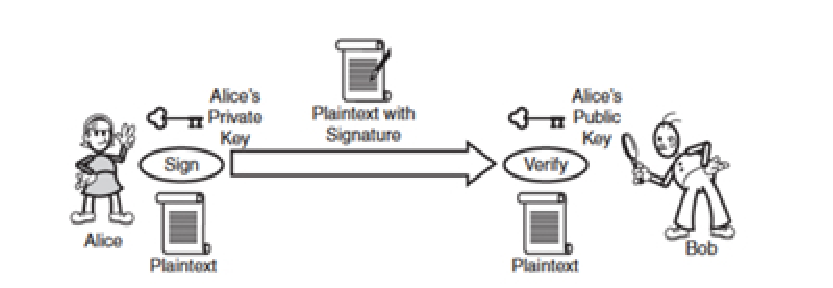
\includegraphics{./Figures/figure14.pdf}
		\rule{35em}{0.5pt}
	\caption[Digital Signature]{Digital Signature. [?]}
	\label{fig:digitalSignature}
\end{figure}

She creates a signature value with her private key and sends it to along with the original plaintext. On the other side, Bob uses Alice's public key to generate a signature value based on the content of the message he received. He then can compare the two signatures to verify the integrity if the incoming message.

\paragraph{Asymmetric versus Symmetric Encryption}

A noticeable caveat of the symmetric encryption is the key distribution problem. Both participants need the same key to encrypt and decrypt a message; therefore they need to somehow exchange it. This has to be done carefully to avoid malicious attackers from stealing the transmitted keys. On the other hand, the most evident downside of the asymmetric encryption is that it exhibits very poor performance. Asymmetric encryption is much slower that symmetric.

\subsubsection{Security protocols}

SSL is probably the most prevalent security protocol for distributing keys in a safe mode. It, essentially, defines the requirements for a secure exchange of keys between two parties. The main steps described by the protocol are the followings:

\begin{enumerate}
  \item 
        The client communicates with a server
  \item 
        The server responds back by returning its certificate
  \item 
        The client computes a random number which represents a seed for generating private keys. He then encrypts this number using the public key included in the server's certificate and sends it to the server.
  \item 
        The server obtains the random number by decrypting the received message
  \item 
        Ultimately, both parties have the same seed; they therefore can create the same private key.
\end{enumerate}

\subsubsection{Public key infrastructure}

As described earlier, in the asymmetric encryption we do not need to bother about how to distribute private keys, since we can share a public key. However, it is critical that we associate the public key with a particular party. In other words, the owner of the public key has to be identified. To that end, the Public Key Infrastructure (PKI) has been designed. The main constituents of PKI are: a certificate, which is a digital resource that associates a participant to a public key. This certificate is digitally signed and issued by a trustworthy third-party authority, which is called Certificate Authority (CA). There is a relatively small number of CAs in PKI and they can issue certificates to other certificate authorities.

To better describe this infrastructure, consider the following example. Figure 1.12 illustrates a typical PKI scenario.

\begin{figure}[htbp]
	\centering
		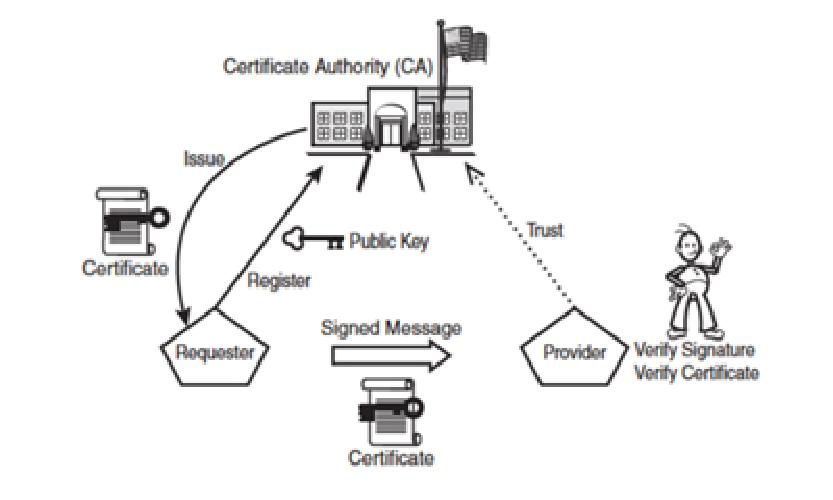
\includegraphics{./Figures/figure15.pdf}
		\rule{35em}{0.5pt}
	\caption[Public Key Infrastructure]{Using certificate for a digital signature. [?]}
	\label{fig:pki}
\end{figure}

Alice signs a message with a private key and sends it to Bob along with a certificate.  Bob creates a signature value using the public key contained in the certificate. But before that, he has to verify that the certificate is signed by a trustworthy certificate authority.

\subsection{Publishing and querying provenance information}

An important task for a provenance-aware system is to capture and store provenance information. An equally crucial feature is to be able for someone to locate that information and ultimately query and retrieve it some format.  For that reason, an infrastructure should be supported so that external applications, users or the application itself could reuse the captured provenance information. Such infrastructure should resolve the problem of locating, retrieving and querying that information. The most appropriate solution is to leverage the current web infrastructure, as well as, some semantic web technologies. In more detail, uniform resource identifiers (URIs) can be assigned to provenance information (provenance-URIs), as well, as, its constituents (i.e. entities, activities and agents). Any application can then perform HTTP GET requests to access the information that is associated with the Uri in question [22]. This is similar to the way URIs are dereferenced when accessing web resources. Nevertheless, it not a strict requirement to assign unique URIs, due to the difficulties that such process has. Thus, alternative methods can be provided to facilitate the same functionality (we discuss them further in this section).

Locating provenance information is crucial and is indispensable in scenarios where a provenance-URI is unknown. In such occasions, an application or a user has to provide some additional information to a provenance provider, which can be a third-party application. According to the submitted information, a provider can locate the provenance-URI and/or the provenance information itself.

Provenance information, as already mentioned, consists of causal relationships between entities, activities, and agents. As such, it is a requirement that one can retrieve descriptions about those resources. The concept is similar, URIs (entity-URIs) can be assigned to those resources and one of the following mechanisms can be provided:

\begin{itemize}
  \item 
        In the case where the requester knows the entity-URI, a simple HTTP mechanism can be used to access the dereferenced content. More specifically, if a resource is accessible via an HTTP GET request, an additional link header denoting the URI where provenance for that resource is located can be injected into the header of the response.
        
\begin{verbatim}
Link: provenance-URI; rel="provenance"; anchor="entity-uri"
\end{verbatim}
        
        The \emph{entity-URI} indicates the location where additional description for that resource can be obtained, whereas the provenance-URI identifies the location of the provenance information which the entity is part of. If the provider though, does not know anything about provenance locations, it can point to a third-party provider or a provenance service. In that case, the link header is slightly different.
        
\begin{verbatim}
Link: provenance-service-URI; rel="provenance-service"; 
anchor="entity-uri"
\end{verbatim}
        
        The \emph{provenance-service-URI} will, essentially, return a service description that will aid a client to locate a provenance-URI or fetch provenance information for the entity in question.
        
  \item 
        For resources that are presented in HTML, provenance-URI can be included within the document. The simplest way to do that would be to use the <Link> html element. Consider the following example.
        
\begin{verbatim}
<html xmlns="http://www.w3.org/1999/xhtml">
    <head>
        <link rel="provenance" href="provenance-URI">
        <link rel="anchor" href="target-URI">
        <title>Welcome to example.com</title>
    </head>
    <body>
       ...
    </body>
</html>
\end{verbatim}
        
        Just as is the case with the previous approach, the document provider can point to a provenance service where the information is stored. In that case the HTML snippet will resemble the following one:
        
\begin{verbatim}
<html xmlns="http://www.w3.org/1999/xhtml">
    <head>
        <link rel="provenance-service" href="service-URI">
        <link rel="anchor" href="target-URI">
        <title>Welcome to example.com</title>
    </head>
    <body>
        ...
    </body>
</html>
\end{verbatim}
  \item 
        Finally, if a resource is represented in one of the several RDF serialization formats (i.e. RDFa, XML/RDF, N-Triples, Turtle etc.) then additional RDF triples can be inserted to describe the provenance of the resource. For this reason, the property \emph{prov:hasProvenance} is defined. The object for that predicate is the resource that contains provenance information about a resource that is subject of this triple.
        
\begin{verbatim}
@prefix prov: <http://www.w3.org/ns/prov#>
<> dcterms:title      "Welcome to example.com" ;
prov:hasAnchor     <http://example.com/data/resource.rdf> ;
prov:hasProvenance <http://example.com/provenance/resource.rdf> ;
prov:hasProvenanceService <http://example.com/provenance-service/> .
  :
(RDF data)
\end{verbatim}

\end{itemize}

\subsubsection{Provenance Services}

There might be occasions where the provenance-URI is unknown. In such cases, a provenance service can provide a means for discovering and/or retrieving provenance information. A provenance service might be supported by a third-party provider, and is uniquely identified via a service-URI. Dereferencing, this URI will bring a service description, which provides guidelines to clients about how to locate or/and fetch provenance information. Two mechanisms are supported to accomplish that task: the provenance discovery service mechanism gets the URI for some resource and returns a set (one or more) of URIs, pointing to the location where the provenance information can be acquired. Conversely, the provenance retrieval service is used when there is no URI associated with the provenance information. As such, the service is responsible for locating and retrieving that information, on client's behalf.

Details about these services are described in the service description, which should be in available as RDF (see example below).

\begin{verbatim}
<service-URI> a prov:ProvenanceService ;
    prov:provenanceUriTemplate "service-URI?target={+uri}" .
\end{verbatim}

The object of the \emph{prov:provenanceUriTemplate} is a literal values that contains a URI template\footnote{J. Gregorio; R. Fielding; M. Hadley; M. Nottingham; D. Orchard. URI Template. March 2012, Internet RFC 6570. URL: http://tools.ietf.org/html/rfc6570}. Users can replace the variable uri with actual uri of the entity for which provenance is required.

An alternative option is to use a query engine. For interoperability's sake, it is preferred that a SPARQL endpoint is used. Requesters can use a simple SPARQL query including an entity-uri, to get the corresponding provenance-uri.

\begin{verbatim}
@prefix prov: http://www.w3c.org/ns/prov#

SELECT ?provenance_uri WHERE
{
  <http://example.org/resource> prov:hasProvenance ?provenance_uri
}

\end{verbatim}

If the requester does not hold any URI, but knows some details about the resource, then those details can be included in the SPARQL query; for example if the DOI identifier for a document is known, then the following query can be submitted to the SPARQL  endpoint:

\begin{verbatim}
@prefix prov: http://www.w3c.org/ns/prov#

@prefix prism: <http://prismstandard.org/namespaces/basic/2.0/>
SELECT ?provenance_uri WHERE
{
  [ prism:doi "1234.5678" ] prov:hasProvenance ?provenance_uri
}
\end{verbatim}

Finally, if specific elements of provenance information are required, then the SPARQL query may look like the following:

\begin{verbatim}
@prefix prov: <http://www.w3c.org/ns/prov#>
SELECT ?generationStartTime WHERE {
    <http://example.org/resource> prov:wasGeneratedBy ?activity .
    ?activity prov:startedAtTime ?generationStartTime .
}

\end{verbatim}

In this example, the client wants to retrieve the start time of an activity in the provenance information in question.

\subsection{Carbon Footprints}

During the last century, human activities brought severe damages to the environment. This has been more evident during the recent years, where anthropogenic environmental impacts have led to severe climate changes [23:1]. To that end, several mechanisms to tackle with this problem need to be devised. In this section we introduce the fundamental terms and concepts that underpin the process of quantifying human's impact on the environment.

\subsubsection{Fundamental Notions}

Carbon footprinting is probably the most prevalent method for quantifying human's impact on the environment. More specifically, the term "footprint" can be associated with quantities of \emph{Greenhouse Gas (GHG)} emissions [Daniel Lashof] caused by activities, individuals, systems or populations. In cases where a more accurate evaluation of climate risk is needed, a measure called \emph{climate footprint} [23:3] can be used. Figure 1.13 illustrates the distinction of those measured. We can notice a third layer which corresponds to a yet broader set of GHGs emissions and is called \emph{GHG inventory}.

\begin{figure}[htbp]
	\centering
		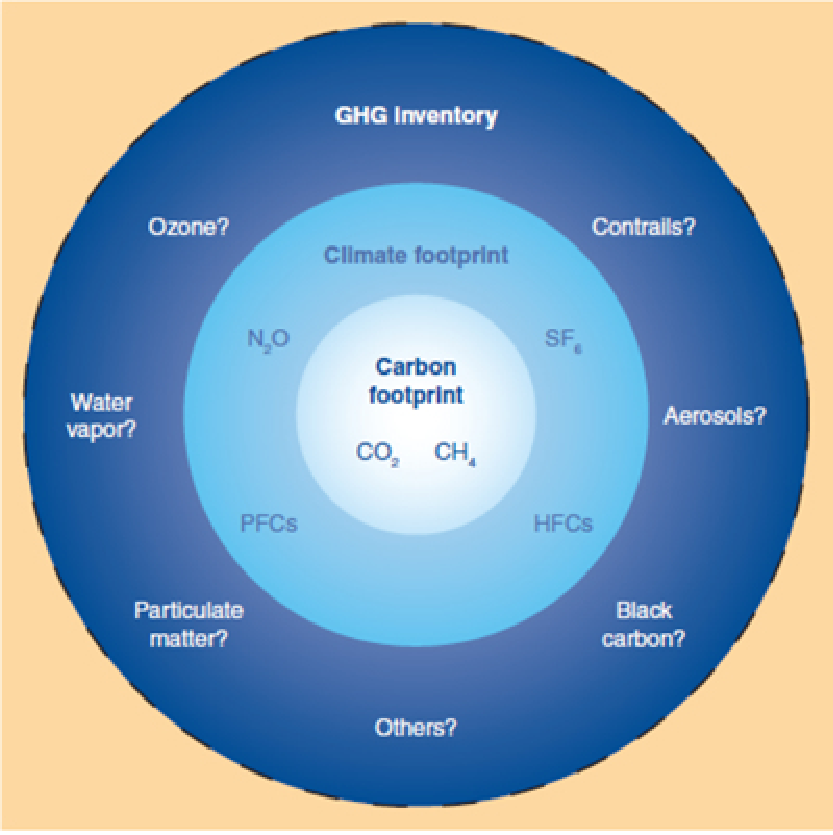
\includegraphics{./Figures/figure16.pdf}
		\rule{35em}{0.5pt}
	\caption[Carbon Emissions Measures]{Three measures for carbon emissions [23]}
	\label{fig:ghgEmissionMeasures}
\end{figure}

\subsubsection{Calculating carbon emissions}

The process of calculating carbon footprints is relatively straightforward and consists of the several steps.

\begin{enumerate}
  \item 
        Initially, all emission sources for the subject need to be compiled and classified; for example, an emission source for an individual might be his daily travels to work with bus.
  \item 
        A method for quantifying the emissions of each source has to be selected. The unit for that quantity is expressed in CO2e, which combines CO2 and CO4 emissions.
  \item 
        All the data that are needed by the method have to be gathered; for example, a method might need some activity data [25] and an appropriate conversion factor (or emission factor); we will come back to these terms in a bit.
  \item 
        A documentation of the method is vital, so that computed values can be validated by re-executing the same method, in the future. Provenance, which we discussed in previous sections, can be a good solution.
\end{enumerate}


\subsubsection{Gathering Emissions Sources}

The carbon footprint calculation process starts by gathering the emissions sources for the subject. To better identify possible emissions sources we can distinguish two types of emissions: direct and indirect emissions.

Direct are the emissions which the subject has full control of. These are the emissions that are primarily produced during the combustion of fossil fuels. On the other hand, indirect emissions are not directly associated with a specific activity, but are due to the demand for products brought by the subject in question; for example, each product that we buy consists of a number of activities that result in the product being on super-markets shelves. Apparently, all these activities cause CO2e emissions. This implies that our demand for products indirectly produced a quantity of CO2e that was emitted to the environment.

\subsubsection{Classifying Emissions}
The prime reason that lies behind the decision for categorizing emissions is the problem of double counting. In essence, it refers to the problem of associating the same quantity of carbon emissions to multiple subjects [23:25]. To avoid this issue, emissions are classified into three distinct scopes.

\begin{description}
  \item[Scope 1]
        In scope 1, the direct carbon emissions of individuals, activities or systems can be found; for example, carbon emissions produced by a car owned by a company.
  \item[Scope 2] 
        Scope 2 consists of emissions that are produced from energy generation. It basically, refers to energy purchased by the subject in question, for own consumption.
  \item[Scope 3] 
        Emissions which are the result of the subject's actions that take place outside the organization or geographic boundaries are scope 3 emissions. In general, this sort of emissions are said to be shared by several subjects rather solely belong to one.
\end{description}


\subsubsection{Calculation Methods}

The next step in calculating emissions is to select an appropriate calculation method, based on the data that are available. The simplest formula suggests that the number of units of the activity that occurred be multiplied by an appropriate conversion factor (emission factor) [23:2]. To better illustrate this concept, imagine that the carbon emissions of a trip made by car needs to be calculated. In that case, we can multiply the distance travelled (or fuel consumed) by a value that define the CO2e emissions of that car per kilometer units.

According to the accuracy and quality of the data that are present, calculation methods can be classified into three categories or tiers; if we choose to use the fuel consumed by a car then several factors that determine the quality of this figure should be considered. The type of the journey, the vehicles age and condition are some of the factors that affect the quantity of fuel consumption. A tier Three method will consider all those factors, as it will use the actual quantity of the fuel used. Further, it will multiply this number by an emission factor published by a government body and which is associated with the particular fuel type. A tier Two method will be less accurate. It will take the distance travelled as the main activity data and multiply it by the emissions factor for the specific car model. Finally, a tier One method will yield the least accurate figure, because it will use the least specific data. In particular, an average distance (published by some government's authority) for that sort of cars will be multiplied by the emission factor associated with that fuel type.

\subsubsection{HEI Scope 3 Carbon Emissions}

In this section we will briefly describe how higher educational institutions (HEI) should calculate scope 3 carbon emissions caused by travels made by the institution's members [24]. First we will remind that scope 3 emissions are those that are caused by sources that are not owned by the HEI. A representative example would be, emissions that are produces by commuting travels by a transport mean that is not owned by the HEI e.g. bus, train etc.

There are two categories of travels: business and commuter travels. The main factor that determines the scope of carbon emissions is the mode of transport that was used; for instance, emissions caused by transport means owned by the HEI are scope 1 emissions. However, travels are often made by modes of transport owned by third-party bodies; hence the corresponding emissions are regarded as scope 3 emissions.

\begin{figure}[htbp]
	\centering
		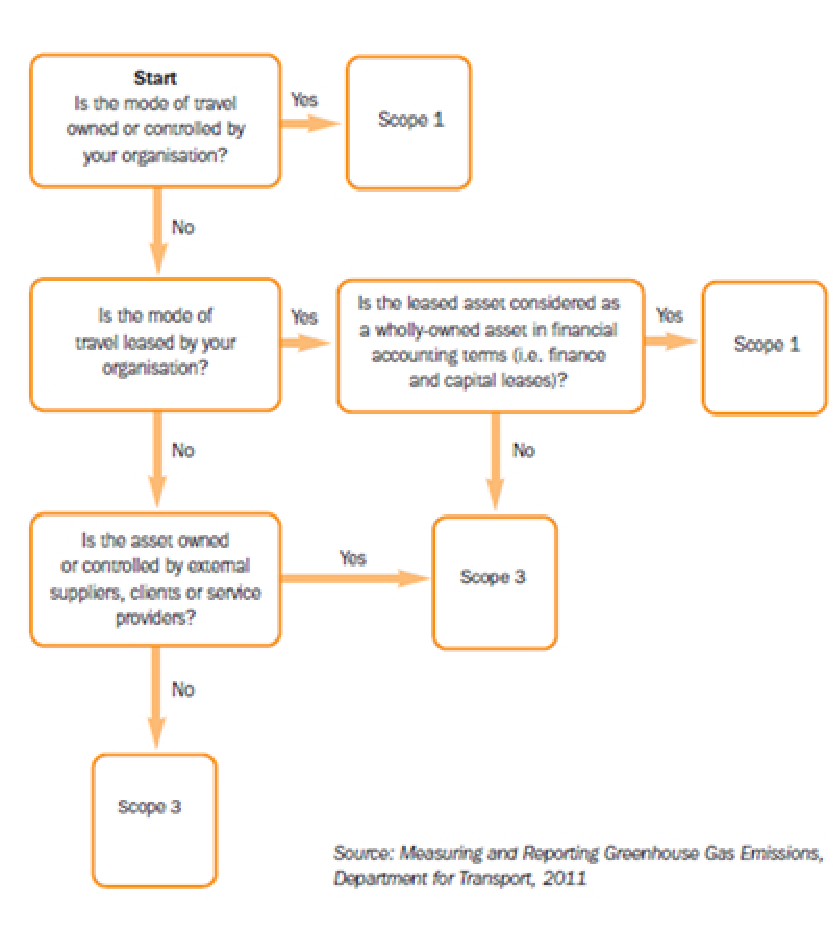
\includegraphics{./Figures/figure17.pdf}
		\rule{35em}{0.5pt}
	\caption[Seperating Scope 1 and Scope 3 Emissions]{How to distinguish scope 1 and scope 3 emissions [24]}
	\label{fig:scope1Scope3}
\end{figure}


\subsubsection{Travel emissions calculation}

The process of calculating emissions caused by travels is the same with what we have presented earlier. As far as travels are concerned, the type of transport mean determines the emission factor that will be used in the calculation formula.


\begin{flushright}
Sunil Patel: \href{http://www.sunilpatel.co.uk}{www.sunilpatel.co.uk}
\end{flushright}
